\documentclass[a4paper, fleqn]{article}
\usepackage{header}

\usetikzlibrary{patterns}
\usepgfplotslibrary{fillbetween}

\title{Семинарский лист 2.3}
\author{
    % Александр Богданов   \\ \href{https://t.me/SphericalPotatoInVacuum}{Telegram} \and
    % Алиса Вернигор       \\ \href{https://t.me/allisyonok}{Telegram} \and
    Анастасия Григорьева \\ \href{https://t.me/weifoll}{Telegram} \and
    % Василий Шныпко       \\ \href{https://t.me/yourvash}{Telegram} \and
    % Данил Казанцев       \\ \href{https://t.me/vserosbuybuy}{Telegram} \and
    Денис Козлов         \\ \href{https://t.me/DKozl50}{Telegram} \and
    Елизавета Орешонок   \\ \href{https://t.me/eaoresh}{Telegram} \and
    Ира Голобородько     \\ \href{https://t.me/Ira4kgl}{Telegram}
    % Иван Пешехонов       \\ \href{https://t.me/JohanDDC}{Telegram} \and
    % Иван Добросовестнов  \\ \href{https://t.me/ivankot13}{Telegram} \and
    % Настя Городилова     \\ \href{https://t.me/nastygorodi}{Telegram} \and
    % Никита Насонков      \\ \href{https://t.me/nnv_nick}{Telegram} \and
    % Сергей Лоптев        \\ \href{https://t.me/beast_sl}{Telegram}
}

\date{Версия от {\ddmmyyyydate\today} \currenttime}

\begin{document}
    \maketitle
    
    \section*{Предполагая функцию $f$ непрерывной на $D$, приведите двойной интеграл от $f$ по $D$ к повторному 
    двумя способами: по $x$ затем по $y$ и наоборот.}
    \subsection*{Задача 1\\[-40 pt]}
    \begin{align*}
        & D = \{ (x, y) \,|\, x, y \in [0; 1], x^2 + y^2 \ge 1 \} \\[3 pt]
        & \text{Множество точек, находящихся в квадрате, ограниченном прямыми $x = 0, x = 1, y = 0, y = 1$,} \\
        & \text{за пределами круга радиуса 1 с центром в точке $(0, 0)$:} \\[3 pt]
    \end{align*}
        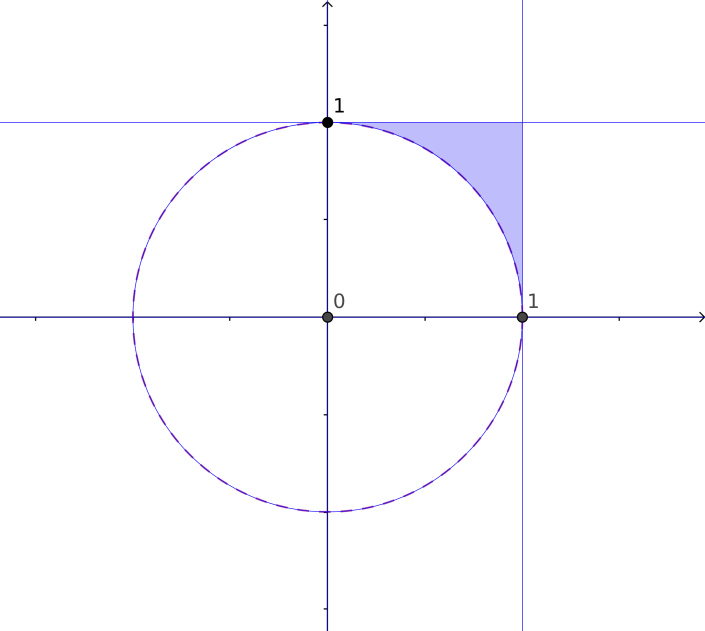
\includegraphics[width=8cm, height=7cm]{task 1.png}\\
    \begin{align*}
        & \text{Интеграл по $x$ затем по $y$:} \\
        & \int\limits_0^1 dy \!\!\! \int\limits_{\sqrt{1-y^2}}^1 \!\!\! dx = \int\limits_0^1 dy \cdot x \Bigm|_{\sqrt{1-y^2}}^1
        = \int\limits_0^1 dy \left( 1 - \sqrt{1-y^2} \right) = \int\limits_0^1 dy - \int\limits_0^1 \sqrt{1-y^2} \, dy 
        = 1 - \int\limits_0^1 \sqrt{1-y^2} \, dy \\
        & \text{Замена: } y = \sin u \Leftrightarrow \int\limits_0^1 \sqrt{1-y^2} \, dy 
        = \int\limits_0^{\frac{\pi}2} \cos u \, \sqrt{1-\sin^2 u} \, du = \int\limits_0^{\frac{\pi}2} \cos^2 u \, du 
        = \int\limits_0^{\frac{\pi}2} \frac{\cos 2u + 1}2 \, du = \\
        & = \frac12 \int\limits_0^{\frac{\pi}2} \cos 2u \, du + \frac12 \int\limits_0^{\frac{\pi}2} \! du 
        = \frac14 \, \sin 2u \Bigm|_0^{\frac{\pi}2} + \frac12\, u \Bigm|_0^{\frac{\pi}2} = \frac{\pi}4 \\
        & \text{Тогда:} \\
        & \int\limits_0^1 dy \!\!\! \int\limits_{\sqrt{1-y^2}}^1 \!\!\! dx = 1 - \frac{\pi}4 \\
        & \text{Очевидно, что повторный интеграл, взятый в другом порядке, будет вычисляться точно так же:} \\
        & \int\limits_0^1 dx \!\!\! \int\limits_{\sqrt{1-x^2}}^1 \!\!\! dy = \int\limits_0^1 dy \cdot y \Bigm|_{\sqrt{1-x^2}}^1
        = \int\limits_0^1 dx \left( 1 - \sqrt{1-x^2} \right) = \int\limits_0^1 dy - \int\limits_0^1 \sqrt{1-x^2} \, dy 
        = 1 - \frac{\pi}4 \\
        & \text{\fbox{Ответ: $1 - \dfrac{\pi}4$.}}
    \end{align*}
    
    \subsection*{Задача 2}
    \begin{align*}
        & D = \{ (x, y) \,|\, x, y \in [0; 1], (x - 1)^2 + (y - 1)^2 \ge 1 \} \\[3 pt]
        & \text{Множество точек, находящихся в квадрате, ограниченном прямыми $x = 0, x = 1, y = 0, y = 1$,} \\
        & \text{за пределами круга радиуса 1 с центром в точке $(1, 1)$:} 
        \end{align*}
        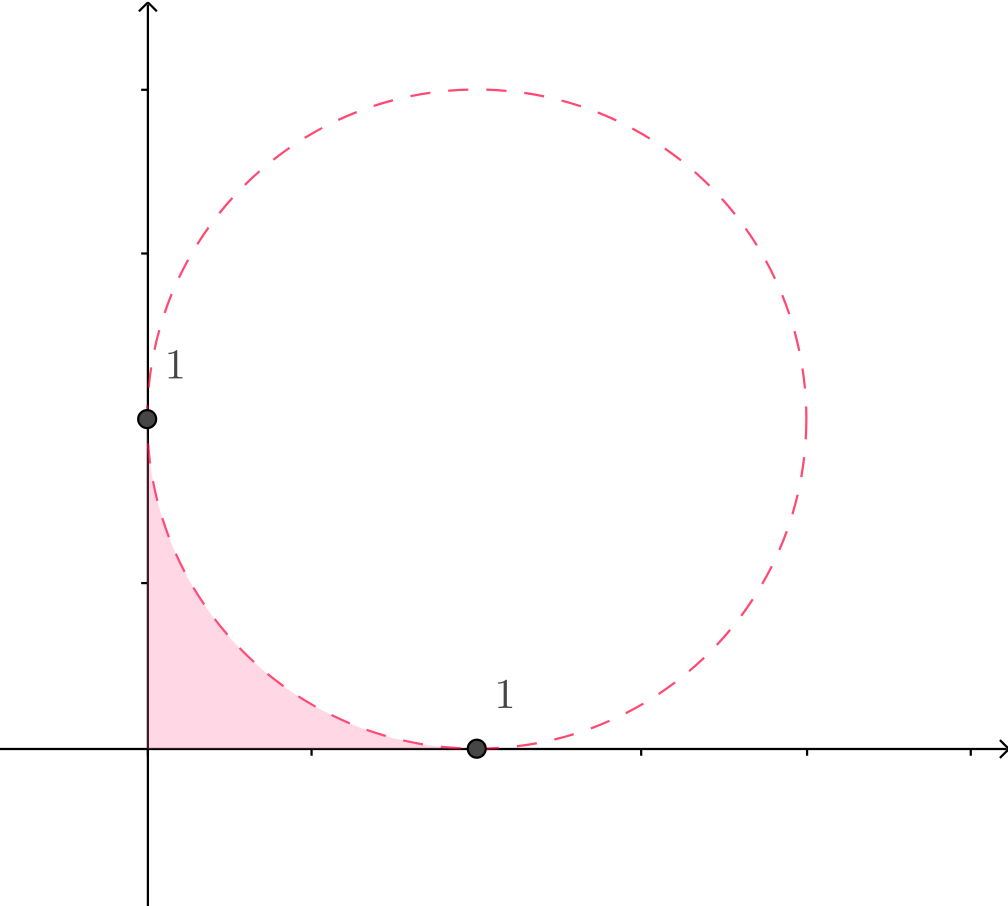
\includegraphics[width=8cm, height=7cm]{task 2.png}\\
        \begin{align*}
        & \text{Интеграл по $x$ затем по $y$:} \\
        & \int\limits_0^1 dy \!\!\! \int\limits_0^{\sqrt{1-(y-1)^2}+1} \!\!\! dx 
        = \int\limits_0^1 dy \cdot x \Bigm|_0^{\sqrt{1-(y-1)^2}+1} = \int\limits_0^1 dy \left( \sqrt{1-(y-1)^2} + 1 \right) 
        = \int\limits_0^1 \sqrt{1-(y-1)^2} \, dy + 1 \\
        & \text{Замена: } (y-1) = \sin u \Leftrightarrow \int\limits_0^1 \sqrt{1-(y-1)^2} \, dy 
        = \int\limits_0^{\frac{\pi}2} \cos u \, \sqrt{1-\sin^2 u} \, du = \int\limits_{-\frac{\pi}2}^0 \cos^2 u \, du 
        = \int\limits_{-\frac{\pi}2}^0 \frac{\cos 2u + 1}2 \, du = \\
        & = \frac12 \int\limits_{-\frac{\pi}2}^0 \cos 2u \, du + \frac12 \int\limits_{-\frac{\pi}2}^0 \! du 
        = \frac14 \, \sin 2u \Bigm|_{-\frac{\pi}2}^0 + \frac12\, u \Bigm|_{-\frac{\pi}2}^0 = -\frac{\pi}4 \\
        & \text{Тогда:} \\
        & \int\limits_0^1 dy \!\!\! \int\limits_0^{\sqrt{1-(y-1)^2}+1} \!\!\! dx = 1 - \frac{\pi}4 \\
        & \text{Очевидно, что повторный интеграл, взятый в другом порядке, будет вычисляться точно так же:} \\
        & \int\limits_0^1 dx \!\!\! \int\limits_0^{\sqrt{1-(x-1)^2}+1} \!\!\! dy = \int\limits_0^1 \sqrt{1-(x-1)^2} \, dx + 1
        = 1 - \frac{\pi}4 \\
        & \text{\fbox{Ответ: $1 - \dfrac{\pi}4$.}}
    \end{align*}
    
    \subsection*{Задача 3}
    
    $D = \{ (x,y ) \mid x^2 + 2 y^2 \leq 16, \; x^2 - y^2 \leq 1\}.$
    
    
    $\bullet$ $ x^2 + 2 y^2 = 16$ -- эллипс, нужны точки внутри него;
    
    $\bullet$ $x^2 - y^2 = 1$ -- гипербола, нужна область, ограниченная двумя частями ее графика. 
    
    
    Найдем координаты точки пересечения кривых: $\begin{cases} x ^ 2 + 2 y^2 = 16;
    x^2  - y^2 = 1;\end{cases} \implies \begin{cases} y = \pm \sqrt{5}; \\ x = \pm \sqrt{6} .\end{cases}$
    
    Эллипс пересекает ось ординат в точках $(0, \sqrt{8})$ и $(0, -\sqrt{8}).$ 
    
    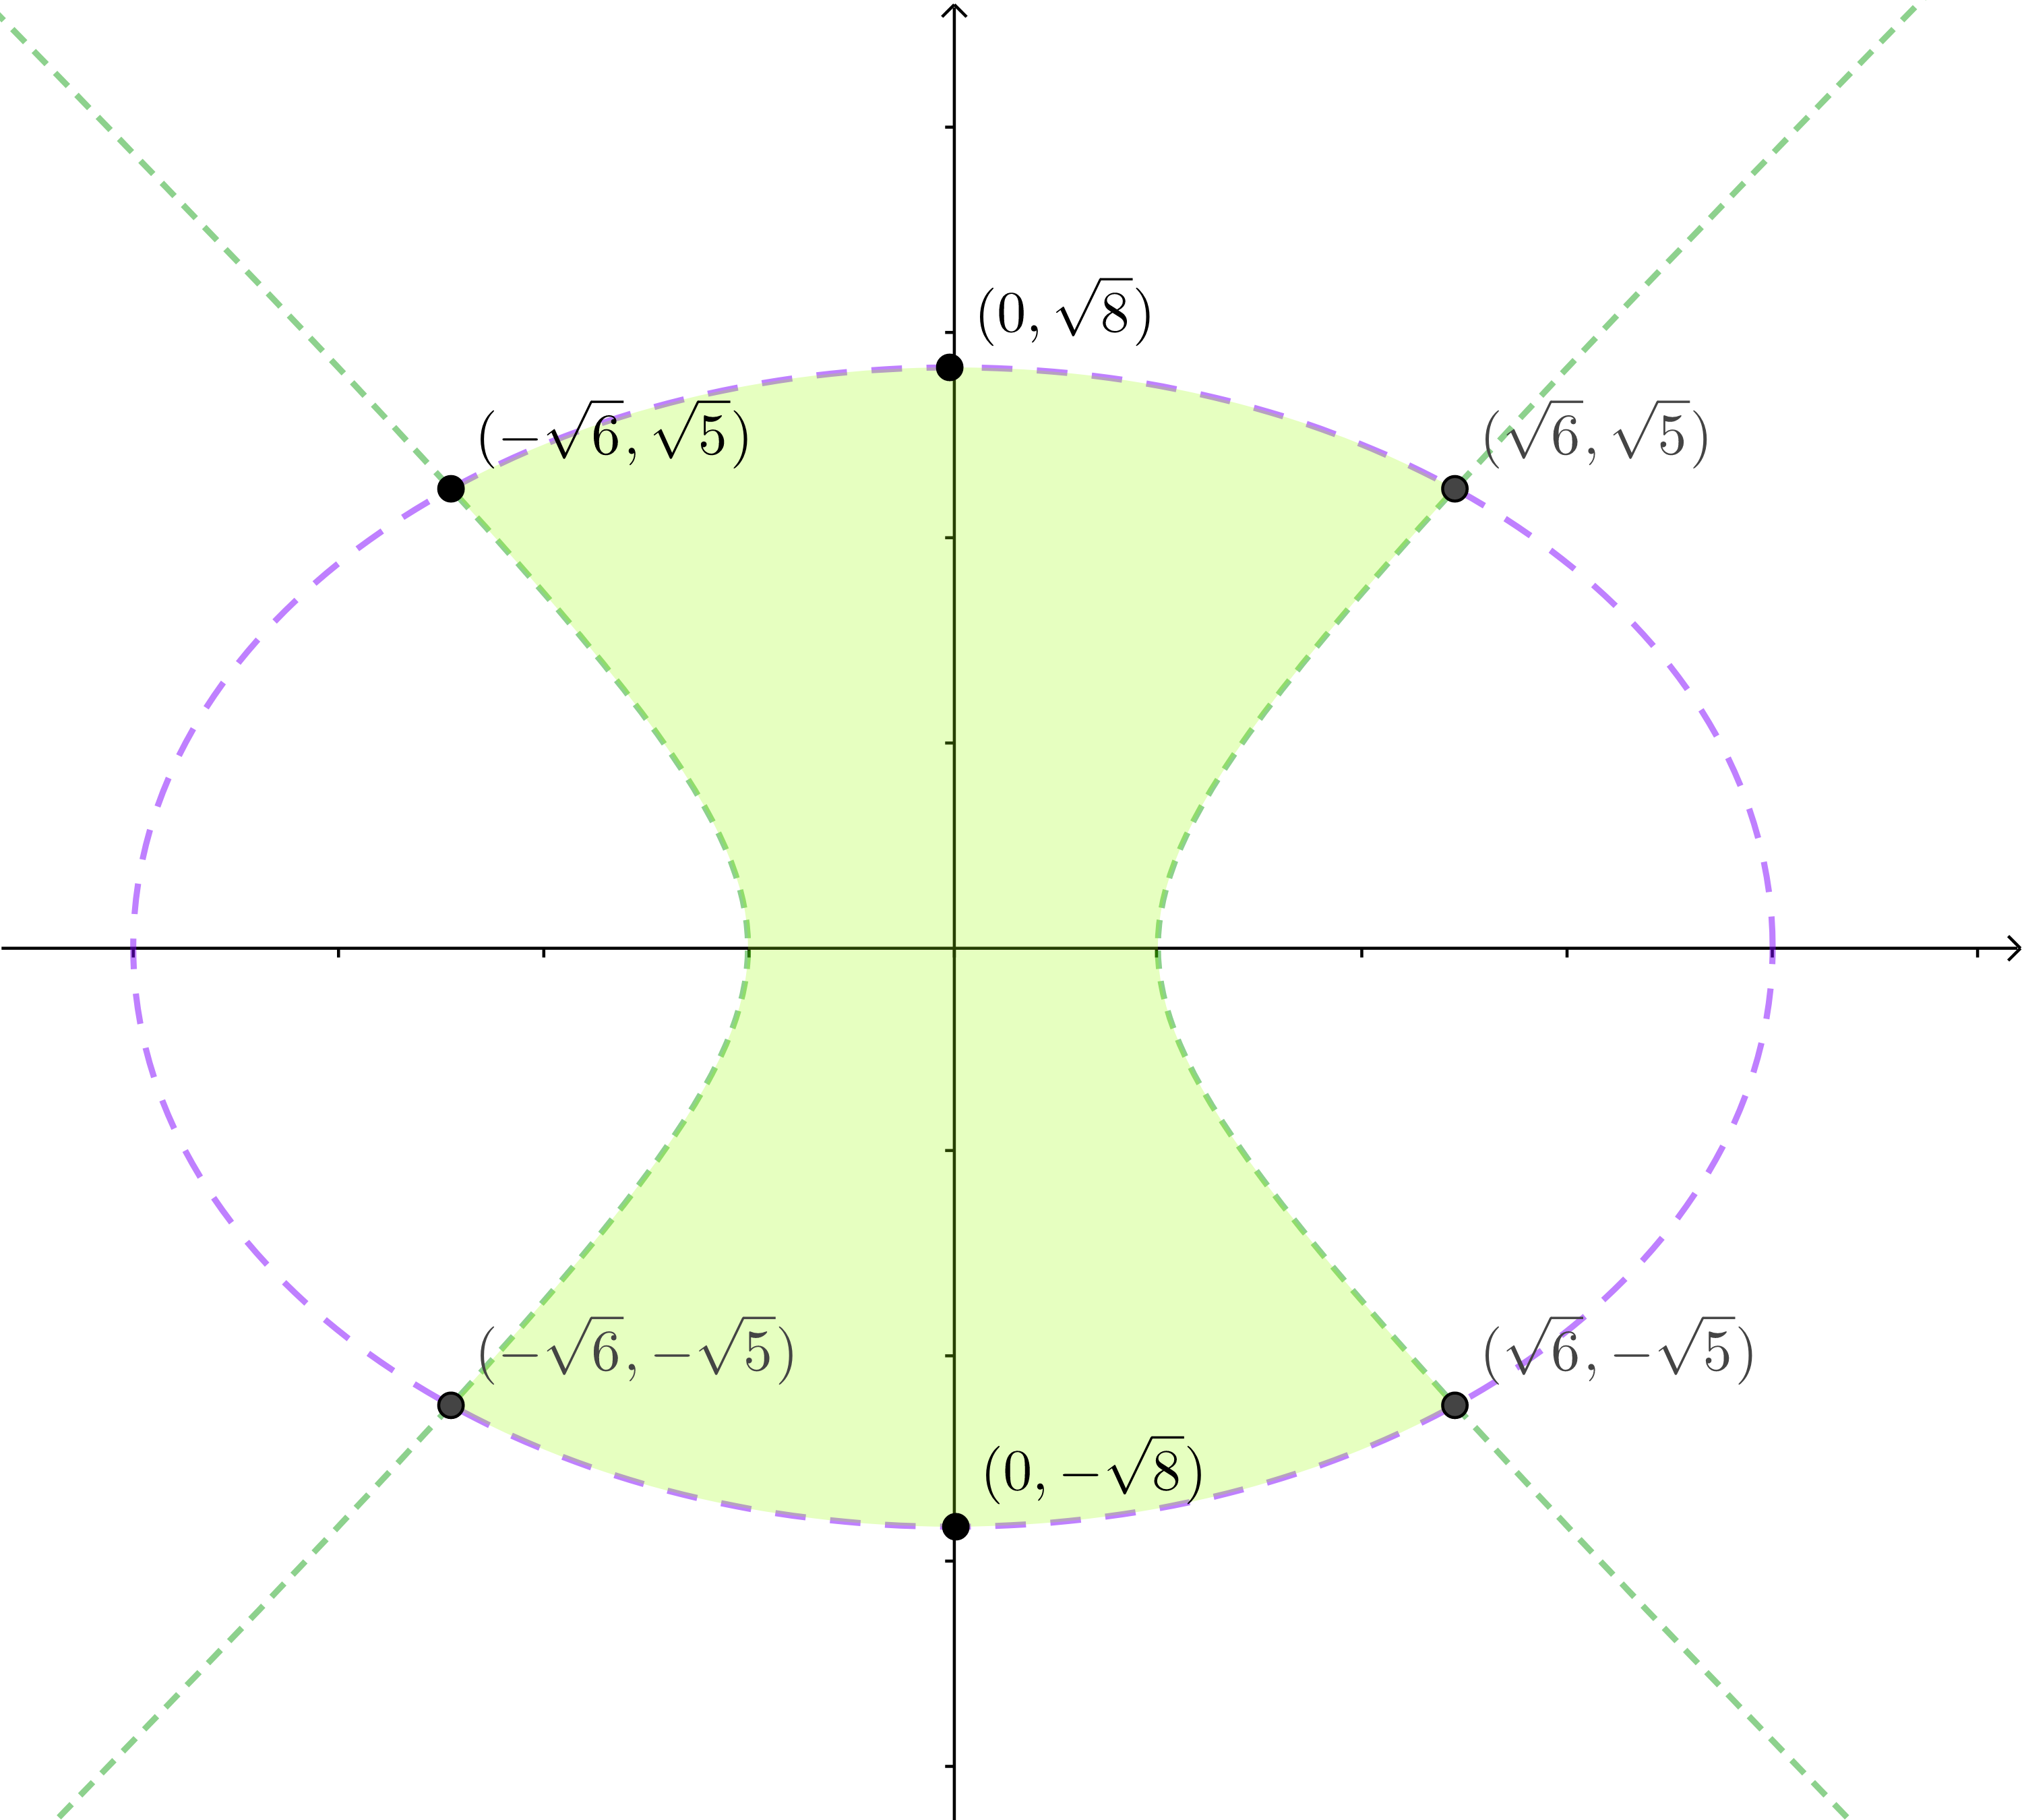
\includegraphics[width=11cm, height=10cm]{task 3.png}
    
    
    Интегрируя по $x$, видим два симметричных относительно 0 куска $\implies$ можем рассмотреть любой из них и продублировать интеграл.
    
    Интегрируем правую часть -- интеграл разбивается на участки до перекрытия гиперболой (до координаты 1) и после. Во втором интеграле используем симметричность относительно $Ox.$
    
    
    
    Итого: $I(D, f) = 2 \cdot \left( \displaystyle \int\limits_0^{1} dx \int\limits_{-\sqrt{(16 - x^2)/2}}^{\sqrt{(16 - x^2)/2} } f(y) dy + 2 \cdot \displaystyle \int\limits_1^{\sqrt{6}} dx \int\limits_{\sqrt{x^2 - 1}}^{\sqrt{(16 - x^2)/2} } f(y) dy \right).$
    
    Теперь по $y$. Тоже используем симметричность и считаем лишь верхнюю часть.
    
     $I(D,f ) = 2 \cdot \left( \displaystyle \int\limits_0^{\sqrt{5}} dy \int\limits_{-\sqrt{1 + y^2}}^{\sqrt{1 + y^2} } f(x) dx + \displaystyle \int\limits_{\sqrt{5}}^{\sqrt{8}} dy \int\limits_{-\sqrt{16 - 2y^2}}^{\sqrt{16 - 2y^2} } f(x) dx \right).$
    
     \subsection*{Задача 4}
        
    $D = \{ (x,y ) \mid x, y \geq 0, \; 0< xy \leq 1, \; y \leq 2x, \; x \leq 2y\}.$
    
    $\bullet$ $xy = 1$ -- гипербола, рассматривается участок под ней;
    
    $\bullet$ $y = 2x$ -- прямая, рассматривается полуплоскость под ней;
    
    $\bullet$ $x = 2y$ -- прямая, рассматривается полуплоскость над ней.
    
    Найдем точки пересечения кривых: $\begin{cases} xy = 1;\\
    y = 2x; \end{cases} \implies\begin{cases} y = \sqrt{2}; \\  x = \sqrt{2}/2 ;\end{cases}\; \; \begin{cases}xy = 1;\\
    x = 2y;\end{cases}\implies\begin{cases}y = \sqrt{2}/2; \\  x = \sqrt{2} .\end{cases}$
    
    Значит, требуется привести интеграл по следующему множеству:
    
    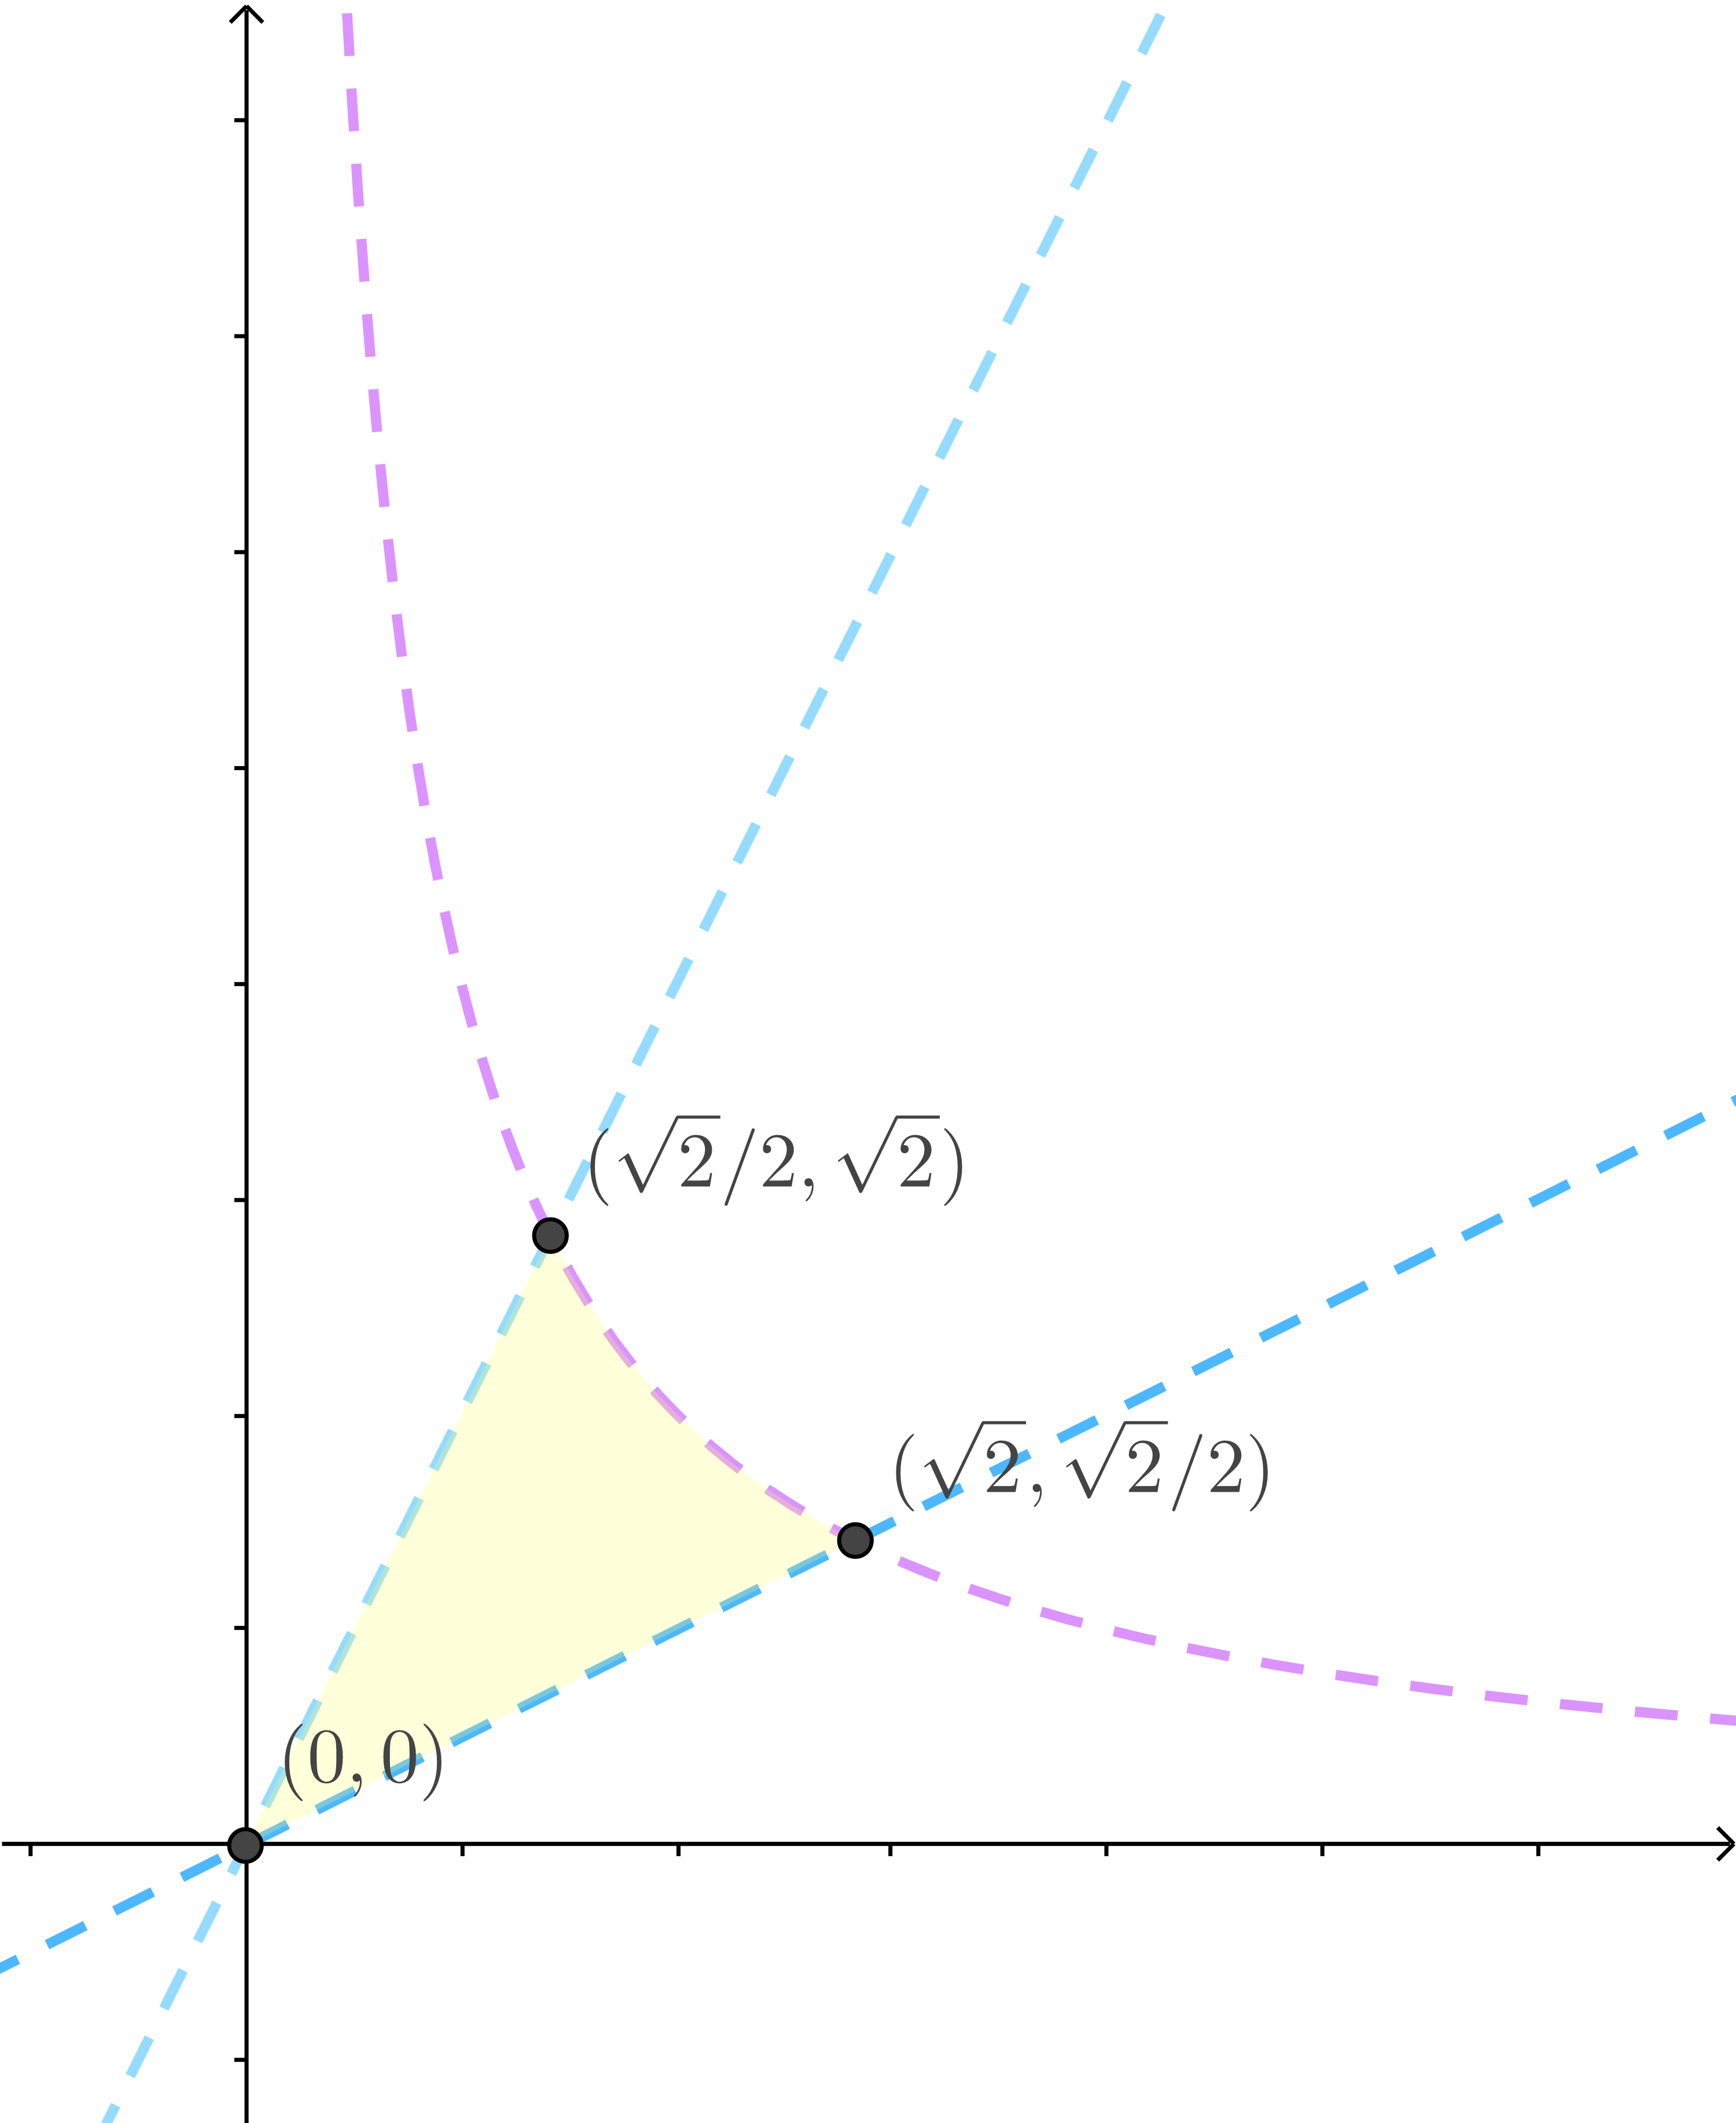
\includegraphics[width=8cm, height=9cm]{task 4.png}
    
    Разбивая область интегрирования по $x$ до перекрытия с гиперболой и после, получаем:
    
    $I(D, f) = \displaystyle \int\limits_{0}^{\sqrt{2}/2}dx \int\limits_{x/2}^{2x} f(y)dy + \displaystyle \int\limits_{\sqrt{2}/2}^{\sqrt{2}}dx \int\limits_{x/2}^{1/x} f(y)dy$;
    
    Разбивая область интегрирования по $y$ до перекрытия с гиперболой и после, получаем (симметрично):
    
    $I(D, f) = \displaystyle \int\limits_{0}^{\sqrt{2}/2}dy \int\limits_{x/2}^{2x} f(x)dx + \displaystyle \int\limits_{\sqrt{2}/2}^{\sqrt{2}}dy \int\limits_{x/2}^{1/x} f(x)dx$.
    
    \section*{Предполагая функцию $f$ непрерывной на $D$, измените порядок интегрирования в повторном интеграле}
    % \subsection*{Задача 5}

    \subsection*{Задача 6}
    \begin{flalign*}
        & \int_0^1 dy \int_{\frac{y^2}{9}}^{y} f(x, y) dx + 
        \int_1^3 dy \int_{\frac{y^2}{9}}^1 f(x, y) dx = \text{ пристально смотрим на рисунок } = \\
        & = \int_0^1 \int_{x}^{3\sqrt{x}} f(x, y) dx dy = 
        \int_0^1 dx \int_{x}^{3\sqrt{x}} f(x, y) dy 
    \end{flalign*}
    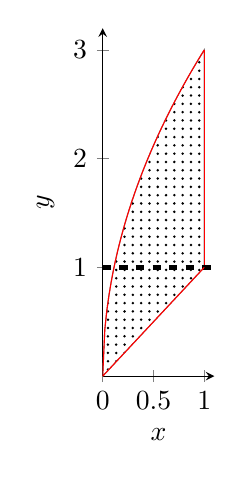
\begin{tikzpicture} 
        \begin{axis}[axis lines=center, xlabel={$x$}, ylabel={$y$}, % служебные строки
                        xlabel near ticks, ylabel near ticks, hide obscured x ticks=false, % служебные строки
                        xmin=0, xmax=1.1, ymin=0, ymax=3.2, % диапазон значений
                        width=3cm, height=6cm] % размер картинки
            % чтобы рисовать линии по координатам (x, y) используйте (axis cs:x, y), как здесь:
            \draw[color=red] (axis cs:1, 1) -- (axis cs:1, 3); % вертикальная линия справа
            \draw[dashed, line width=2pt, color=black] (axis cs:0, 1) -- (axis cs:1.1, 1); % деление двух интегралов
            % чтобы заполнить площадь между графиками стоит дать графикам имена (здесь A и B):
            \addplot [name path=A, domain=0:1, color=red] {x}; 
            \addplot [name path=B, domain=0:1, color=red, samples=50] {sqrt(x)*3}; % тикз умеет в математику
            \addplot [pattern=dots, draw=gray] fill between[of=A and B]; % само заполнение через fill between
        \end{axis} 
    \end{tikzpicture} 

    % \subsection*{Задача 7}
    
    % \subsection*{Задача 8}
    
    \section*{Изменив порядок интегрирования, вычислите интеграл}
    % \subsection*{Задача 9}
    
    \subsection*{Задача 10}
    \begin{flalign*}
        & \int_0^2 x^2 dx \int_x^2 \ln(1 + y^2) dy = \text{ пристально смотрим на рисунок } = 
        \int_0^2 \int_0^y x^2 \ln(1 + y^2) dx dy = \\
        & = \int_0^2 \ln(1 + y^2) dy \int_0^y x^2 dx =
        \int_0^2 \ln(1 + y^2) dy \left( \left. \frac{x^3}{3} \right|_0^y \right) = 
        \frac{1}{3} \int_0^2 \ln(1 + y^2) y^3 dy = \\
        & = \left\{ \begin{array} {ll}
            u = \ln(1 + y^2) & \Rightarrow u' = \frac{2y}{1 + y^2} \\
            v' = y^3 & \Rightarrow v = \frac{y^4}{4} 
        \end{array}  \right\} = 
        \frac{1}{3} \left. \ln(1 + y^2) \frac{y^4}{4} \right|^2_0 -
        \frac{1}{3} \int_0^2 \frac{y^4}{4} \frac{2y}{1 + y^2} dy = 
        \left\{ \begin{array} {l}
            t = 1 + y^2 \\
            dt = 2y dy \\
            dy = \frac{dt}{2y} 
        \end{array}  \right\} = \\
        & = \frac{1}{3} \left( 4 \ln(5) - 0 \right) - \frac{1}{6} \int_1^5 \frac{y^5}{t} \frac{dt}{2y} = 
        \frac{4}{3} \ln(5) - \frac{1}{12} \int_1^5 \frac{(y^4 + 2y^2 + 1) - (2y^2 - 2) + 1}{t} dt = \\
        & = \frac{4}{3} \ln(5) - \frac{1}{12} \int_1^5 \frac{t^2 - 2t + 1}{t} dt = 
        \frac{4}{3} \ln(5) - \frac{1}{12} \left( \int_1^5 t dt - 2 \int_1^5 dt + \int_1^5 \frac{dt}{t}  \right) = \\
        & = \frac{4}{3} \ln (5) - \frac{1}{12} \left( \left( \frac{25}{2} - \frac{1}{2} \right) -
        2 (5 - 1) + \ln(|t|)\big|^5_1 \right) = \frac{4}{3} \ln(5) - \frac{1}{12} \left( 12 - 8 + \ln(5) \right) = \\
        & = \frac{4}{3} \ln(5) - \frac{1}{3} - \frac{\ln(5)}{12} = \pmb{\frac{5\ln(5)}{4} - \frac{1}{3}}
        % \frac{1}{3} \int_0^2 \frac{y^4}{4} y^3 dy = \\
        % & = \frac{1}{3} \left( 4 \ln(5) - 0 \right) - \frac{1}{12} \left. \frac{y^8}{8} \right|^2_0 =
        % \frac{4}{3} \ln(5) - \frac{8}{3} 
    \end{flalign*}
    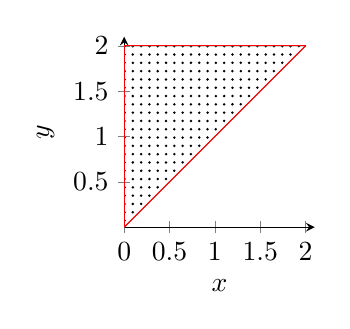
\begin{tikzpicture} 
        \begin{axis}[axis lines=center, xlabel={$x$}, ylabel={$y$},
                        xlabel near ticks, ylabel near ticks, hide obscured x ticks=false,
                        xmin=0, xmax=2.1, ymin=0, ymax=2.1,
                        width=4cm, height=4cm]
            \draw[color=red] (axis cs:0, 0) -- (axis cs:0, 2);
            \addplot [name path=A, domain=0:2, color=red] {2}; 
            \addplot [name path=B, domain=0:2, color=red, samples=50] {x}; 
            \addplot [pattern=dots, draw=gray] fill between[of=A and B];
        \end{axis} 
    \end{tikzpicture} 
    
    % \subsection*{Задача 11}
    
    % \subsection*{Задача 12}
    
    \section*{Вычислите интеграл}
    % \subsection*{Задача 13}
    
    \subsection*{Задача 14}
    
    % \subsection*{Задача 15}
    
    % \subsection*{Задача 16}
    
    \section*{Предполагая функцию $f$ непрерывной на $D$, измените порядок интегрирования в повторном интеграле
    всеми возможными способами}
    % \subsection*{Задача 17}
    
    \subsection*{Задача 18}
    
    % \subsection*{Задача 19}
    
    % \subsection*{Задача 20}
    
    % \subsection*{Задача 21}
    
    % \subsection*{Задача 22}
    
\end{document}
